% Contribution for the pinned ProveIt manuscript continuation.
% Dependencies: amsmath, amssymb, amsthm, booktabs, hyperref.
% The root article supplies theorem/proposition/lemma/corollary environments.
% Existing manuscript labels are referenced only where explicitly stated.

\section{The first classical failure of saturation: the fifth index}
\label{n5:sec:transition}\label{sec:classical-zeros}

The first four Stieltjes indices in the baseline have the maximum possible
number of positive parameter-derivative zeros at every derivative order.
That pattern fails at the next index.  The failure is not restricted to a
Lerch deformation: it occurs at the classical Hurwitz endpoint itself.
We prove the exact transition
\begin{equation}\label{n5:eq:count-sequence}
 \#\{a>0:\gamma_5^{(k)}(a)=0\}=
 \begin{cases}3,&k=1,2,\\5,&k\geq3,\end{cases}
\end{equation}
and every zero in this display is simple.  Thus the least derivative order
after which fifth-index saturation persists is exactly three.

Two ingredients distinguish this conclusion from a numerical zero scan.
A general upper bound of five controls the entire positive axis at order
three.  Certified signs at its stationary points then count the zeros at
orders two and one by monotonicity.  The large positive zeros near
$148.9122$ and $319.6184$ are essential to this argument; a scan confined to
a small neighborhood of $a=1$ misses them.

\subsection{Endpoint signs, parity, and monotonicity of zero counts}

Retain the Laurent convention
\[
 \zeta(s,a)=\frac1{s-1}+
       \sum_{n\geq0}\frac{(-1)^n}{n!}\gamma_n(a)(s-1)^n,
 \qquad a>0.
\]
For the classical family write
\[
 U_{n,k}(a)=(-1)^{n+k}\gamma_n^{(k)}(a),\qquad k\geq1.
\]
Then $U_{n,k}'=-U_{n,k+1}$.  The established Appell--Laplace formula is
\begin{equation}\label{n5:eq:laplace}
 U_{n,k}(a)=\int_0^\infty
 \frac{t^k e^{-at}}{1-e^{-t}}\,Q_n(\log t)\,dt,
 \qquad
 \frac{e^{xz}}{\Gamma(1+z)}=
       \sum_{n\geq0}Q_n(x)\frac{z^n}{n!}.
\end{equation}
The reciprocal-gamma product makes $Q_n$ strictly real-rooted, and Laplace
variation diminution therefore bounds the positive zero count by $n$,
including multiplicities.  These are the baseline's global zero theorem
and its proof mechanism, reproduced in Section~\ref{sec:zero-preliminaries}
for completeness.  The classical parameter-derivative identity underlying
\eqref{n5:eq:laplace} is also contained in Coffey's all-order
formulas~\cite{Coffey}.

For fixed $n\geq0$ and $k\geq1$ the endpoint expansions are
\begin{align}
 U_{n,k}(a)&\sim k!a^{-k-1}\log^n(1/a),&&a\downarrow0,\label{n5:eq:left}\\
 U_{n,k}(a)&\sim(-1)^n(k-1)!a^{-k}\log^n a,&&a\to\infty.
 \label{n5:eq:right}
\end{align}
When $n=0$, the logarithmic powers mean one.  The first formula follows
either by scaling the integral or by differentiating the shift term
$\log^n a/a$ in
$\gamma_n(a)=\log^n a/a+\gamma_n(a+1)$.  For the second, set $t=u/a$ in
\eqref{n5:eq:laplace} and use
$(1-e^{-u/a})^{-1}=a/u+O(1+u/a)$ together with monicity of $Q_n$.
The bound
$(1-e^{-v})^{-1}\leq1+v^{-1}$ supplies an integrable majorant after
expanding the fixed polynomial in $\log u-\log a$.
In particular, every $U_{n,k}$ tends to zero at infinity and has fixed
strict signs near both endpoints.

\begin{proposition}[Parity and persistence before saturation]
\label{n5:prop:count}
Let $N_{n,k}$ be the total multiplicity of the positive zeros of
$\gamma_n^{(k)}$.  Then
\begin{equation}\label{n5:eq:count-law}
 0\leq N_{n,k}\leq n,\qquad
 N_{n,k}\equiv n\pmod2,\qquad N_{n,k+1}\geq N_{n,k}.
\end{equation}
Consequently every strict increase in the total zero count is by an even
integer.  The same assertions hold, at each fixed
$0\leq\rho\leq1$, for the baseline Stieltjes--Lerch family
$D_{n,k}^{\rho}$.
\end{proposition}
\begin{proof}
The upper bound is the global variation theorem.  The endpoint signs in
\eqref{n5:eq:left}--\eqref{n5:eq:right} show that the total multiplicity
has parity $n$: a real analytic zero reverses sign exactly when its
multiplicity is odd.

Suppose the distinct zeros of $U_{n,k}$ are
$r_1<\cdots<r_q$, with multiplicities $m_1,\ldots,m_q$ and
total $N=\sum_i m_i>0$.  Its derivative has inherited multiplicity
$m_i-1$ at each $r_i$, and Rolle's theorem supplies a zero between each
successive pair.  These account for at least
$(N-q)+(q-1)=N-1$ derivative zeros counted with multiplicity.  There is one
more stationary point strictly after $r_q$: a nonzero function leaving
zero at $r_q$, with constant sign afterwards and limit zero at infinity,
must attain an interior extremum.  Thus $U_{n,k+1}=-U_{n,k}'$ has at least
$N$ zeros counted with multiplicity.  The case $N=0$ is immediate.

For fixed $\rho<1$, the analogous Mellin weight
$(1-\rho e^{-t})^{-1}$ is positive and tends to $(1-\rho)^{-1}$ at zero.
The large-$a$ leading term is then
$(-1)^n k!(1-\rho)^{-1}a^{-k-1}\log^n a$; the small-$a$ leading term
is unchanged.  The same endpoint and Rolle arguments apply, including
the possible multiple zeros at $\rho=0$.
\end{proof}

\begin{proposition}[A classical lower bound from matching endpoint data]
\label{n5:prop:lower}
For every $k\geq1$, $\gamma_n^{(k)}$ has at least two distinct positive
zeros if $n\geq2$ is even, and at least three distinct positive zeros if
$n\geq3$ is odd.  In particular, saturation for $n=2,3$ at every
derivative order follows analytically, without a finite sign certificate.
\end{proposition}
\begin{proof}
For $n\geq2$, the shift identity at $a=1$ and its first derivative give
\[
 \gamma_n(1)=\gamma_n(2),\qquad
 \gamma_n'(1)=\gamma_n'(2),\qquad
 \int_1^2\gamma_n'(a)\,da=0.
\]
Put $g=\gamma_n'$.  This is a nonzero real analytic function.  If its
common endpoint value is positive, its integral forces a negative
interior value; hence there are at least two sign-changing zeros in
$(1,2)$.  The same conclusion holds with signs reversed when the common
endpoint value is negative.  If the common endpoint value is zero, the
integral forces both signs in the interior, and there are at least three
distinct zeros in $[1,2]$, including the endpoints.

For odd $n$ in the nonzero-endpoint case, the two interior sign-changing
zeros have odd multiplicities.  The odd total parity from
Proposition~\ref{n5:prop:count} forces an additional odd-multiplicity
zero, distinct from them.  This proves the asserted lower bounds at
$k=1$.  Rolle's theorem between distinct zeros, together with the
stationary point after the last zero used above, preserves a lower bound
on the number of distinct zeros at every subsequent derivative order.
The global upper bound makes the two or three zeros simple when
$n=2$ or $n=3$.
\end{proof}

Thus the count three in \eqref{n5:eq:count-sequence} is the smallest
possible classical fifth-index count.  Passing from order two to order
three raises the positive zero count by exactly two.

\subsection{A finite certificate that controls the whole positive axis}

For the remainder of the proof abbreviate
\[
 U_k=U_{5,k},\qquad
 V_k(a)=\frac{a^{k+1}}{k!}U_k(a).
\]
The normalization $V_k$ preserves signs, but its stationary points are
not the zeros of $U_{k+1}$.  All monotonicity arguments below are applied
to $U_k$, while $V_k$ is used only for stable sign enclosures.

Let $\varepsilon=10^{-16}$.  Each row of
Table~\ref{n5:tab:roots} specifies a rational interval
$[\ell,\ell+\varepsilon]$.  The stated endpoint signs of $V_k$ are
certified by the outward computation proved in the next subsection.

\begin{table}[htbp]
\centering
\small
\begin{tabular}{ccrcc}
\toprule
$k$&$j$&$\ell$&sign at $\ell$&sign at $\ell+10^{-16}$\\
\midrule
3&1&0.9409528529131887&$+$&$-$\\
3&2&1.1292935180347063&$-$&$+$\\
3&3&1.6357795548293846&$+$&$-$\\
3&4&6.1361342793896981&$-$&$+$\\
3&5&319.6184025568026870&$+$&$-$\\
\midrule
2&1&1.3713298168772550&$+$&$-$\\
2&2&1.9113619446041762&$-$&$+$\\
2&3&148.9122045692035618&$+$&$-$\\
\midrule
1&1&1.1378900542449414&$+$&$-$\\
1&2&1.6389372768448503&$-$&$+$\\
1&3&2.1249028498579805&$+$&$-$\\
\bottomrule
\end{tabular}
\caption{Rational isolating intervals of width $10^{-16}$.  These
endpoint signs and the critical-value signs in the next table are finite
certificates.  The proof establishes uniqueness and completeness.}
\label{n5:tab:roots}
\end{table}

Denote the five third-order roots by $c_1<\cdots<c_5$ and the three
second-order roots by $d_1<d_2<d_3$.  The interval computation also
encloses the preceding-order function uniformly on every indicated
root interval.  Table~\ref{n5:tab:critical} lists rational enclosures
with outward rounding; they apply in particular at the true roots.

\begin{table}[htbp]
\centering
\small
\begin{tabular}{cl}
\toprule
Quantity&Certified rational enclosure\\
\midrule
$V_2(c_1)$&$[0.006154632340,\ 0.006154632341]$\\
$V_2(c_2)$&$[0.041073722584,\ 0.041073722585]$\\
$V_2(c_3)$&$[-0.097090480335,\ -0.097090480334]$\\
$V_2(c_4)$&$[106.545043234228,\ 106.545043234229]$\\
$V_2(c_5)$&$[-135615.425337743697,\ -135615.425337743695]$\\
\midrule
$V_1(d_1)$&$[-0.014754703693,\ -0.014754703692]$\\
$V_1(d_2)$&$[0.028710652775,\ 0.028710652776]$\\
$V_1(d_3)$&$[-466915.576951780840,\ -466915.576951780837]$\\
\bottomrule
\end{tabular}
\caption{Signs of the lower-order function at every critical point.
The verifier encloses the function on the entire rational root bracket,
so these signs do not presume a floating-point approximation to a root.}
\label{n5:tab:critical}
\end{table}

\begin{theorem}[The exact fifth-index transition]
\label{n5:thm:transition}
The positive zero counts are exactly those in
\eqref{n5:eq:count-sequence}.  All zeros are simple.  The eleven
intervals in Table~\ref{n5:tab:roots} isolate all zeros at derivative
orders one, two, and three.  For every $k\geq3$, the five zeros at order
$k+1$ strictly interlace to the right of those at order $k$.
\end{theorem}
\begin{proof}
The five third-order interval signs give at least five distinct zeros of
$U_3$.  The global upper bound of five, counting multiplicity, shows that
they are all its positive zeros and that each is simple.  Starting with
the positive left endpoint sign, the signs of $U_3$ on the six
complementary intervals are
\[
  +,\ - ,\ +,\ -,\ +,\ -.
\]
Consequently $U_2'=-U_3$ has constant nonzero sign on each such
interval.  Its values at the five critical points have signs
\[
 \operatorname{sgn}(U_2(c_1),\ldots,U_2(c_5))=(+,+,-,+,-).
\]
Therefore there is exactly one second-order zero in each of
$(c_2,c_3)$, $(c_3,c_4)$, and $(c_4,c_5)$, and no zero in
$(0,c_1)$ or $(c_1,c_2)$.  After $c_5$, the function $U_2$ is strictly
increasing from a negative value to its limit zero, so there is no zero
there either.  The three zeros lie away from the critical points, so
each is simple.  Their brackets in Table~\ref{n5:tab:roots} consequently
identify them as $d_1,d_2,d_3$.

The signs of $U_2$ are now $+,-,+,-$ on the four intervals cut out by
the $d_j$, and $U_1'=-U_2$.  The critical-value signs are $-,+,-$.
Since $U_1$ is positive near zero, strict monotonicity gives exactly one
zero in each of $(0,d_1)$, $(d_1,d_2)$, and $(d_2,d_3)$.  After $d_3$,
$U_1$ increases from a negative value to zero, so it has no further
zero.  Again all three crossings are simple.

Finally, five simple zeros at order three force at least five distinct
zeros at the next order: Rolle supplies four between adjacent roots
and the vanishing tail supplies one after the last root.  The global
upper bound gives exactly five simple zeros, with no additional zero
before the first interval.  Repeating proves saturation and strict
right interlacing for every $k\geq3$.
\end{proof}

\begin{figure}[htbp]
\centering
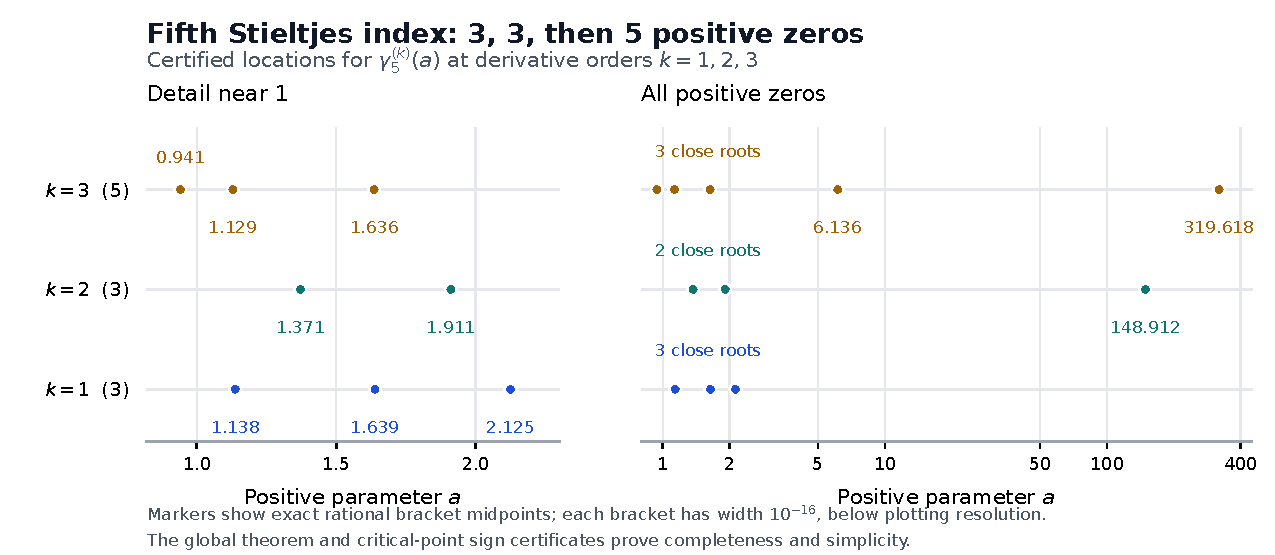
\includegraphics[width=\textwidth]{figures/n5_certified_zero_locations.pdf}
\caption{The eleven certified zero locations. The local panel separates the near-unit roots; the logarithmic panel includes the large roots. The brackets have width $10^{-16}$, much smaller than a plotted marker.}
\label{fig:n5-locations}
\end{figure}

This proof uses no claim that a dense set of sampled values accounts for
every zero.  Completeness at the highest checked order comes from a
global analytic theorem; completeness at lower orders comes from the
complete list of stationary points and their certified signs.

\subsection{Rational Euler--Maclaurin verification}

The certificate is self-contained in
\texttt{certify\_n5\_zeros.py}.  It uses only Python's standard-library
integer and rational arithmetic.  Its output
\texttt{n5\_zero\_certificates.json} records all integer endpoints,
the analytic error bounds, and the assertions that the relevant
intervals exclude zero.  The following derivation specifies its
mathematical contract.

Define exact rational coefficients by
\[
 \prod_{j=1}^{r}(1+z/j)=\sum_i e_i(r)z^i,
 \qquad
 R_{n,r}(v)=n!\sum_{i=0}^{\min(n,r)}
                  e_i(r)\frac{(-v)^{n-i}}{(n-i)!}.
\]
The spectral representation is
\begin{equation}\label{n5:eq:spectral}
 V_{n,k}(a):=\frac{a^{k+1}U_{n,k}(a)}{k!}
   =\sum_{m\geq0}\left(\frac a{a+m}\right)^{k+1}
             R_{n,k}(\log(a+m)).
\end{equation}
In the three orders used here,
\begin{align*}
 R_{5,1}(v)&=-v^5+5v^4,\\
 R_{5,2}(v)&=-v^5+\frac{15}{2}v^4-10v^3,\\
 R_{5,3}(v)&=-v^5+\frac{55}{6}v^4-20v^3+10v^2.
\end{align*}
Higher $r$ in the error analysis use the same exact recurrence, without
numerically evaluating zeta or gamma functions.

For positive rational $a$, choose integers $M,R\geq1$, put $p=k+1$,
$A=a+M>1$, $v=\log A$, and $L=k+2R$.  Set
\begin{align}
 E_{M,R}={}&\sum_{m=0}^{M-1}
       \left(\frac a{a+m}\right)^pR_{n,k}(\log(a+m))\notag\\
 &+\left(\frac aA\right)^p
       \left[\frac Ak R_{n,k-1}(v)+\frac12R_{n,k}(v)\right]\notag\\
 &+\left(\frac aA\right)^p\sum_{r=1}^{R}
    \frac{B_{2r}}{(2r)!}\frac{(k+1)_{2r-1}}{A^{2r-1}}
       R_{n,k+2r-1}(v),\label{n5:eq:EM}
\end{align}
where $(b)_j$ is the rising factorial.  Then
\begin{align}
 |V_{n,k}(a)-E_{M,R}|&\leq
 \left(\frac aA\right)^p\frac{|B_{2R}|}{(2R)!}
       \frac{(k+1)_{2R-1}}{A^{2R-1}}\,\mathcal B_{n,L}(v),
       \label{n5:eq:EM-error}\\
 \mathcal B_{n,L}(v)&=
 \sum_{i=0}^{\min(n,L)}\sum_{j=0}^{n-i}
       \frac{n!e_i(L)}{(n-i-j)!L^j}v^{n-i-j}.
       \label{n5:eq:EM-majorant}
\end{align}
Every factor in the latter bound is nonnegative.

For clarity, the periodic-Bernoulli error estimate in
\eqref{n5:eq:EM-error} is sufficient; no first-omitted-term sign assertion
is needed.  With
$f(x)=x^{-k-1}R_{n,k}(\log x)$, direct coefficient differentiation gives
\[
 f^{(q)}(x)=(-1)^q(k+1)_q x^{-k-q-1}
                            R_{n,k+q}(\log x).
\]
The integral of $f$ from $A$ to infinity is
$A^{-k}R_{n,k-1}(\log A)/k$, which produces the integral term in
\eqref{n5:eq:EM}.  Euler--Maclaurin through the $R$th Bernoulli
correction gives the remaining terms.  Its remainder is bounded by
$|B_{2R}|/(2R)!$ times $a^{k+1}\int_A^\infty|f^{(2R)}(x)|\,dx$.
Majorize $R_{n,L}$ by its coefficientwise absolute values at
$\log x>0$ and use
\[
 \int_A^\infty x^{-L-1}\log^d x\,dx
  =\frac{A^{-L}}{L}
        \sum_{j=0}^{d}\frac{d!}{(d-j)!L^j}\log^{d-j}A.
\]
The leading $L$ cancels the last factor of $(k+1)_{2R}$, yielding
exactly \eqref{n5:eq:EM-error}--\eqref{n5:eq:EM-majorant}.

For logarithms, reduce a positive rational argument to $2^b y$ with
$1\leq y<2$, set $u=(y-1)/(y+1)$, and use
\begin{equation}\label{n5:eq:log-error}
 0\leq\log y-2\sum_{j=0}^{T-1}\frac{u^{2j+1}}{2j+1}
 \leq\frac{2u^{2T+1}}{(2T+1)(1-u^2)}.
\end{equation}
The same formula with $y=2$ encloses $\log2$.  Exact rational
Bernoulli numbers come from their finite triangular recurrence, while
the $e_i(r)$ come from multiplying the finite products above.

The executed parameters are
\[
       n=5,\quad M=24,\quad R=16,\quad T=120,
       \qquad\hbox{fixed denominator }10^{80}.
\]
Every addition, multiplication, division, and integer power is rounded
outwards at this denominator.  The largest analytic
Euler--Maclaurin error bound among all thirty enclosures is less than
$2.591\times10^{-32}$.  This statement concerns the analytic truncation
error; the separate rational interval widths also include all arithmetic
rounding and, where appropriate, the uncertainty across a root bracket.
The final signs are proved by the complete intervals, not by comparing
only the analytic error with a floating-point value.

The code checks twenty-two endpoint signs and eight uniform
critical-point signs.  Evaluating the same interval formulas with
$a$ ranging over a rational interval remains valid by ordinary interval
arithmetic and monotonicity of the logarithm.  This is how
Table~\ref{n5:tab:critical} certifies values at roots without assigning
an exact value to a numerical approximation.

\subsection{Consequences and further questions}

The baseline correctly limited its all-order small-index theorem to
$n\leq4$.  The new fifth-index theorem therefore resolves its first
explicitly open small-order case, rather than correcting a theorem
already stated with the necessary restriction.  It rules out extending
the conclusion to all $n$ at every $k\geq1$.

Several precise continuation questions now replace that false
extrapolation.  Determine the classical saturation threshold
\[
 K_n^{\mathrm{cl}}=
   \min\{k\geq1:N_{n,k}=n\text{ and all positive zeros are simple}\}.
\]
The present results give $K_n^{\mathrm{cl}}=1$ for $1\leq n\leq4$
and $K_5^{\mathrm{cl}}=3$.  Monotonicity and parity constrain every
possible count sequence, while the concentration theorem guarantees an
eventual threshold at each fixed index.  An effective upper bound in
terms of the extreme Appell-root spacing would turn this qualitative
fact into a terminating certified search.

The descending critical-value method applies beyond the fifth index:
once one derivative order is globally saturated and its roots are
isolated, uniform enclosures of the preceding derivative at those
critical points determine the complete lower-order zero count.  It is
particularly useful when the positive roots span several orders of
magnitude.  The count sequence need not increase at every step; the
plateau $3,3$ followed by $5$ is already an exact example.

Finally, quantify how the additional classical zeros arise as the Lerch
parameter increases from zero to one.  The lower bound in
Proposition~\ref{n5:prop:lower} uses exact unit-shift endpoint identities
at the classical endpoint and does not hold for arbitrary $\rho<1$.
This gives a structural reason to study branch creation as well as the
motion of existing simple zeros.
